\documentclass[aspectratio=169,c]{beamer} % 16:9 top adjusted

\usepackage[english]{babel}
\usetheme{Darmstadt} % Mertens: Madrid
%\usecolortheme[options]{beamer color theme}

%\setbeamerfont{title}{series=\bfseries, family=\rmfamily}
%\setbeamercolor{title}{fg=white, bg=red!50!black}
%\setbeamertemplate{navigation symbols}{}


\usepackage{tikz}
\usetikzlibrary{snakes, backgrounds, fit, shapes.geometric, calc}
\usepackage{amsmath}
\usepackage{amssymb}
\usepackage{algorithmic}
\usepackage{algorithm}
%\node [fill=black!30, ellipse fit= (t) (c) (d)]{};
\newcommand{\tikzmark}[1]{\tikz[overlay,remember picture] \node (#1) {};}
\newcommand{\AddBraceTop}[4]{%
    \begin{tikzpicture}[overlay, remember picture]
        \draw [decoration={brace,amplitude=0.5em},decorate,ultra thick,#4]
        (#1.north east) --
        (#2.south -| #1.north east) % (#1.x, #2.y)
        node[midway,right=0.5em,align=left,text width=2.5cm] {#3};
    \end{tikzpicture}%
}
\newcommand{\AddBraceTopShift}[5]{%
    \begin{tikzpicture}[overlay, remember picture]
        \draw [decoration={brace,amplitude=0.5em},decorate,ultra thick,#4]
        ($(#1.north east) + #5$) --
        ($(#2.south -| #1.north east) + #5$) % (#1.x, #2.y)
        node[midway,right=0.5em,align=left,text width=2.5cm] {#3};
    \end{tikzpicture}%
}
\newcommand{\AddBraceBottom}[4]{%
    \begin{tikzpicture}[overlay, remember picture]
        \draw [decoration={brace,amplitude=0.5em},decorate,ultra thick,#4]
        (#1.north -| #2.south east) -- % (#2.x, #1.y)
        (#2.south east)
        node[midway,right=0.5em,align=left,text width=2.5cm] {#3};
    \end{tikzpicture}%
}
\newcommand{\AddBraceReverseShift}[6]{%
    \begin{tikzpicture}[overlay, remember picture]
        \draw [decoration={brace,amplitude=0.5em},decorate,ultra thick,#4]
        ($(#2.south -| #1.north west) + #5$) -- % (#1.x, #2.y)
        ($(#1.north west) + #5$)
        node[midway,right=#6,align=left,text width=2.5cm] {#3};
    \end{tikzpicture}%
}
\newcommand{\AddTextShift}[4]{%
    \begin{tikzpicture}[overlay, remember picture]
        \draw ($(#1.north west) + #4$) -- ($(#1.north west) + #4$)
        node[right=0.5em,align=left,text width=4cm, #3] {#2};
    \end{tikzpicture}%
}
\newcommand{\AddArrowNorth}[4]{%
    \begin{tikzpicture}[overlay, remember picture]
        \draw [-{stealth},ultra thick,#3]
        ($(#1) + #4$) node[right=0em,align=left,text width=2.5cm] {#2} 
        -- (#1.north);
    \end{tikzpicture}%
}
\newcommand{\AddArrowSouth}[4]{%
    \begin{tikzpicture}[overlay, remember picture]
        \draw [-{stealth},ultra thick,#3]
        ($(#1) + #4$) node[right=0em,align=left,text width=2.5cm] {#2} 
        -- (#1.south);
    \end{tikzpicture}%
}

\title{Flows}
\subtitle{Proseminar Algorithmen auf Graphen}
\author{Nils Wagner}
\institute{RWTH Aachen University}
\date{\today}


\begin{document}
\begin{frame}[plain]
    \maketitle
\end{frame}

\begin{frame}{Table of Contents}
    \tableofcontents
\end{frame}

%\section{Concept}
%\begin{frame}{Concept II (optimizations)}
%    \begin{enumerate}
%        \item Flow Networks
%        \begin{itemize}
%            \item introductory example (water pipes/transportation) for intuitive understanding
%            \item definition flow network, capacity, flow, value of flow, max flow problem
%        \end{itemize}
%        \item Ford Fulkerson Method
%        \begin{itemize}
%            \item residual network, residual capacity (example and defintion)
%            \item augmenting path, augmentation (and cancellation) (example)
%            \item algorithm in pseudo code and demonstration
%            \item proof of correctness: intuitive explanation with example (incl. cuts superficially)
%        \end{itemize}
%        \item Running Time: DFS vs.~BFS (Edmond-Karp)
%        \item Capacity Scaling
%        \begin{itemize}
%            \item idea, algorithm and demonstration, running time
%        \end{itemize}
%        \item Dinic's algorithm
%        \begin{itemize}
%            \item idea, algorithm and demonstration, running time
%        \end{itemize}
%        \item Push-Relabel algorithms
%        \begin{itemize}
%            \item idea, demonstration \& correctness, running time
%        \end{itemize}
%    \end{enumerate}
%\end{frame}

%\begin{frame}{additional ideas}
%    \begin{itemize}
%        \item using flow networks to solve bipartite matching problem (outlook at the end or up to 3-4 slides)
%        \begin{itemize}
%            \item (what is bipartite matching)
%            \item example problem
%            \item mapping bipartite matching problem to max-flow problem
%            \item varying capacities and meaning in context
%        \end{itemize}
%        \item example problem with solution/link to github repo with implementations in different languages (Java, Python, C, Haskell, (Prolog))
%    \end{itemize}
%\end{frame}

% beginning of presentation
\section{Flow Networks and Maximum-Flow Problem}
\begin{frame} % introductory slide
    \begin{columns}[c]
        \begin{column}{0.5\linewidth}
            Consider the following problem: 
            \begin{itemize}[<+->]
                \item production facility \(s\) \visible<12->{\alert<12>{\textit<13->{\color<13->{blue!80}(source)}}}
                \item rail network through cities \(A\), \(B\), \(C\), \(D\), \(s\)\visible<3->{, and \(t\)} \visible<11->{\alert<11>{\textit<12->{\color<12->{blue!80}(flow network)}}}
                \item destination \(t\) \visible<12->{\alert<12>{\textit<13->{\color<13->{blue!80}(sink)}}}
                \item limited amount of goods per day from one city to another \visible<13->{\alert<13>{\textit<14->{\color<14->{blue!80}(capacity)}}}
                \item How many goods can be transported from \(s\) to \(t\) per day? \visible<14->{\alert<14>{(maximum flow)}}
                % \item How many goods can be transported from \(s\) to \(t\) per day? \visible<14->{\alert<14>{\textit<15->{(maximum flow)}}} % for handout
            \end{itemize}
        \end{column}
        \begin{column}<6->{0.5\linewidth}
            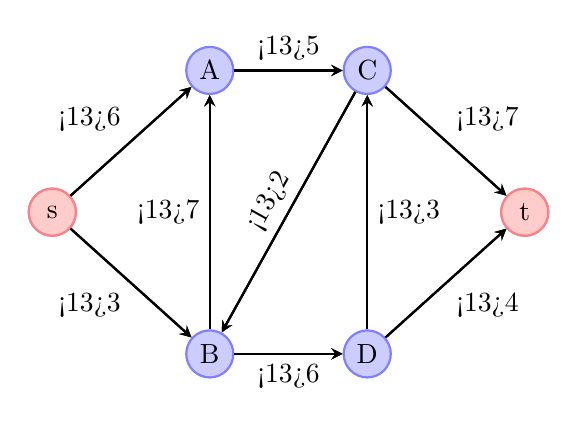
\begin{tikzpicture}
                [x=10mm, y=9mm, 
                nsty/.style={circle, draw=blue!50, fill=blue!20, thick, inner sep=0.15em, minimum size=1.7em},
                rsty/.style={circle, draw=red!50, fill=red!20, thick, inner sep=0.15em, minimum size=1.7em},
                asty/.style={-{stealth}, thick}]
                % nodes
                \visible<6->{\node[nsty] (s) at (-2,0) {s};}
                \visible<7->{\node[nsty] (a) at (0,2)  {A};}
                \visible<7->{\node[nsty] (b) at (0,-2) {B};}
                \visible<7->{\node[nsty] (c) at (2,2)  {C};}
                \visible<7->{\node[nsty] (d) at (2,-2) {D};}
                \visible<8->{\node[nsty] (t) at (4,0)  {t};}
                \visible<12>{\node[rsty] (s) at (-2,0) {s};}
                \visible<12>{\node[rsty] (t) at (4,0)  {t};}
                % edges without capacities
                \visible<9>{\draw[asty] (s) to (a);}
                \visible<9>{\draw[asty] (s) to (b);}
                \visible<9>{\draw[asty] (b) to (a);}
                \visible<9>{\draw[asty] (a) to (c);}
                \visible<9>{\draw[asty] (b) to (d);}
                \visible<9>{\draw[asty] (c) to (b);}
                \visible<9>{\draw[asty] (d) to (c);}
                \visible<9>{\draw[asty] (c) to (t);}
                \visible<9>{\draw[asty] (d) to (t);}
                % adding capacities
                \visible<10->{\draw[asty] (s) -- node[auto]      {\only<13>{\color{red}}6} (a);}
                \visible<10->{\draw[asty] (s) -- node[auto, swap]{\only<13>{\color{red}}3} (b);}
                \visible<10->{\draw[asty] (b) -- node[auto]      {\only<13>{\color{red}}7} (a);}
                \visible<10->{\draw[asty] (a) -- node[auto]      {\only<13>{\color{red}}5} (c);}
                \visible<10->{\draw[asty] (b) -- node[auto, swap]{\only<13>{\color{red}}6} (d);}
                \visible<10->{\draw[asty] (c) -- node[midway, sloped, above]{\only<13>{\color{red}}2} (b);}
                \visible<10->{\draw[asty] (d) -- node[auto, swap]{\only<13>{\color{red}}3} (c);}
                \visible<10->{\draw[asty] (c) -- node[auto]      {\only<13>{\color{red}}7} (t);}
                \visible<10->{\draw[asty] (d) -- node[auto, swap]{\only<13>{\color{red}}4} (t);}
            \end{tikzpicture}
        \end{column}
    \end{columns}
\end{frame}

\begin{frame} % definition flow network
    \begin{columns}[c]
        \begin{column}{0.5\linewidth}
            \begin{Definition}[Flow Network]
                \visible<1->{A {\color<1>{red}\color<2->{blue!80}flow network} \(G=(V,E)\) is a directed graph.}

                \visible<2->{The vertices \(s,t\in V\) are called the {\color<2>{red}\color<3->{blue!80}source} and the {\color<2>{red}\color<3->{blue!80}sink} of \(G\).}

                \visible<3->{The {\color<3>{red}capacity function} \(c: V\times V\to \mathbb R_{\geq 0}\) assigns capacities to the edges of \(G\) where \(c(u,v)=0\) for all \((u,v)\not\in E\).}
            \end{Definition}
        \end{column}
        \begin{column}{0.5\linewidth}
            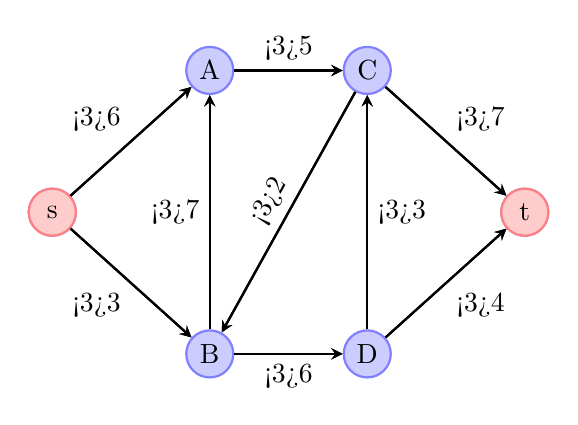
\begin{tikzpicture}
                [x=10mm, y=9mm, 
                nsty/.style={circle, draw=blue!50, fill=blue!20, thick, inner sep=0.15em, minimum size=1.7em},
                rsty/.style={circle, draw=red!50, fill=red!20, thick, inner sep=0.15em, minimum size=1.7em},
                asty/.style={-{stealth}, thick}]
                % nodes
                \node[nsty] (s) at (-2,0) {s};
                \node[nsty] (a) at (0,2)  {A};
                \node[nsty] (b) at (0,-2) {B};
                \node[nsty] (c) at (2,2)  {C};
                \node[nsty] (d) at (2,-2) {D};
                \node[nsty] (t) at (4,0)  {t};
                \visible<2>{\node[rsty] (s) at (-2,0) {s};}
                \visible<2>{\node[rsty] (t) at (4,0)  {t};}
                % edges without capacities
                \draw[asty] (s) to (a);
                \draw[asty] (s) to (b);
                \draw[asty] (b) to (a);
                \draw[asty] (a) to (c);
                \draw[asty] (b) to (d);
                \draw[asty] (c) to (b);
                \draw[asty] (d) to (c);
                \draw[asty] (c) to (t);
                \draw[asty] (d) to (t);
                % adding capacities
                \draw[asty] (s) -- node[auto]      {\only<3>{\color{red}}6} (a);
                \draw[asty] (s) -- node[auto, swap]{\only<3>{\color{red}}3} (b);
                \draw[asty] (b) -- node[auto]      {\only<3>{\color{red}}7} (a);
                \draw[asty] (a) -- node[auto]      {\only<3>{\color{red}}5} (c);
                \draw[asty] (b) -- node[auto, swap]{\only<3>{\color{red}}6} (d);
                \draw[asty] (c) -- node[midway, sloped, above]{\only<3>{\color{red}}2} (b);
                \draw[asty] (d) -- node[auto, swap]{\only<3>{\color{red}}3} (c);
                \draw[asty] (c) -- node[auto]      {\only<3>{\color{red}}7} (t);
                \draw[asty] (d) -- node[auto, swap]{\only<3>{\color{red}}4} (t);
            \end{tikzpicture}
        \end{column}
    \end{columns}
\end{frame}

\begin{frame} % flow and value of flow
    \begin{columns}[c]
        \begin{column}{0.5\linewidth}
            \begin{definition}<1->[Flow and Value of Flow]
                \visible<3->{A function \(f: V\times V\to\mathbb R\) is called a {\color<3->{blue!80}flow} in the network \(G=(V,E)\) if it satisfies the following properties:}
                \vspace*{1mm}
                \begin{enumerate}[<4->]
                    \itemsep 2mm
                    \item \visible<4->{\(0 \leq f(u,v) \leq c(u,v) \forall u,v,\in V\) \color<4->{blue!80}(capacity constraint)}
                    \item \visible<5->{\(\sum\limits_{v\in V}\!f(u,v)=\!\sum\limits_{v\in V}\!f(v,u)\forall u\in V\setminus\{s,t\}\)\newline \color<5->{blue!80}(flow conservation)}
                \end{enumerate} \vspace*{0.2cm}
                \visible<8->{The {\color<8->{blue!80}value of a flow} \(\lvert f\rvert\) is given by 
                \vspace*{-2mm}
                \begin{equation*}
                    \lvert f \rvert =\sum\limits_{v\in V}f(s,v)-\sum\limits_{v\in V}f(v,s).
                \end{equation*}}
                \vspace*{-2mm}
            \end{definition}
        \end{column}
        \begin{column}<1->{0.5\linewidth}
            \begin{tikzpicture}
                [x=10mm, y=9mm, 
                nsty/.style={circle, draw=blue!50, fill=blue!20, thick, inner sep=0.15em, minimum size=1.7em},
                rsty/.style={circle, draw=red!50, fill=red!20, thick, inner sep=0.15em, minimum size=1.7em},
                asty/.style={-{stealth}, thick}]
                % nodes
                \visible<1->{\node[nsty] (s) at (-2,0) {s};}
                \visible<1->{\node[nsty] (a) at (0,2)  {A};}
                \visible<1->{\node[nsty] (b) at (0,-2) {B};}
                \visible<1->{\node[nsty] (c) at (2,2)  {C};}
                \visible<1->{\node[nsty] (d) at (2,-2) {D};}
                \visible<1->{\node[nsty] (t) at (4,0)  {t};}
                \visible<6-7>{\node[rsty] at (0,-2) {B};}
                \visible<6-7>{\node[rsty] at (2,-2) {D};}
                % vertices
                \visible<1>{\draw[asty] (s) -- node[auto]{6} (a);}
                \visible<1>{\draw[asty] (s) -- node[auto, swap]{3} (b);}
                \visible<1>{\draw[asty] (b) -- node[auto]{7} (a);}
                \visible<1>{\draw[asty] (a) -- node[auto]{5} (c);}
                \visible<1>{\draw[asty] (b) -- node[auto, swap]{6} (d);}
                \visible<1>{\draw[asty] (c) -- node[midway, sloped, above]{2} (b);}
                \visible<1>{\draw[asty] (d) -- node[auto, swap]{3} (c);}
                \visible<1>{\draw[asty] (c) -- node[auto]{7} (t);}
                \visible<1>{\draw[asty] (d) -- node[auto, swap]{4} (t);}
                % adding flow
                \visible<2->{\draw[asty] (s) -- node[auto]      {\only<2>{\color{red}}\only<2->{5}\only<2>{\color{black}}/6} (a);}
                \visible<2->{\draw[asty] (s) -- node[auto, swap]{\only<2>{\color{red}}\only<2->{2}\only<2>{\color{black}}/3} (b);}
                \visible<2->{\draw[asty] (b) -- node[auto]      {\only<2>{\color{red}}\only<2->{0}\only<2>{\color{black}}/7} (a);}
                \visible<2->{\draw[asty] (a) -- node[auto]      {\only<2>{\color{red}}\only<2->{5}\only<2>{\color{black}}/5} (c);}
                \visible<2->{\draw[asty] (b) -- node[auto, swap]{\only<2,7>{\color{red}}\only<2-6>{5}\only<7->{4}\only<2,7>{\color{black}}/6} (d);}
                \visible<2->{\draw[asty] (c) -- node[midway, sloped, above]{\only<2>{\color{red}}\only<2->{2}\only<2>{\color{black}}/2} (b);}
                \visible<2->{\draw[asty] (d) -- node[auto, swap]{\only<2>{\color{red}}\only<2->{1}\only<2>{\color{black}}/3} (c);}
                \visible<2->{\draw[asty] (c) -- node[auto]      {\only<2>{\color{red}}\only<2->{4}\only<2>{\color{black}}/7} (t);}
                \visible<2->{\draw[asty] (d) -- node[auto, swap]{\only<2>{\color{red}}\only<2->{3}\only<2>{\color{black}}/4} (t);}
            \end{tikzpicture}
            \visible<9->{
                \begin{align*}
                    \lvert f\rvert &= \sum_{v\in V}f(s,v)-\sum_{v\in V}f(v,s) \\
                    &= \quad 5 + 2 \quad\; - \quad 0\quad\qquad = 7
                \end{align*}}
        \end{column}
    \end{columns}
\end{frame}

\begin{frame}{Maximum-Flow Problem}
    \begin{Problem}<1->%{maximum-flow problem}
        \centering
        Given a flow network \(G\) with source \(s\), sink \(t\), and a capacity function \(c\). 
        
        Find a flow \(f\) in \(G\) of maximum value.
    \end{Problem}
    \begin{columns}[T]
        \begin{column}<2->{0.5\linewidth}
            Applications:
            \begin{itemize}
                \item water flowing through network of pipes/rivers
                \item current in electrical network
                \item traffic: cars in road network
                \item messages in telecommunication network
            \end{itemize}
        \end{column}
        \begin{column}<3->{0.5\linewidth}
            \vspace*{-0.35cm}
            \begin{tikzpicture}
                [x=10mm, y=9mm, 
                nsty/.style={circle, draw=blue!50, fill=blue!20, thick, inner sep=0.15em, minimum size=1.7em},
                rsty/.style={circle, draw=red!50, fill=red!20, thick, inner sep=0.15em, minimum size=1.7em},
                asty/.style={-{stealth}, thick}]
                % nodes
                \visible<3->{\node[nsty] (s) at (-2,0) {s};}
                \visible<3->{\node[nsty] (a) at (0,2)  {A};}
                \visible<3->{\node[nsty] (b) at (0,-2) {B};}
                \visible<3->{\node[nsty] (c) at (2,2)  {C};}
                \visible<3->{\node[nsty] (d) at (2,-2) {D};}
                \visible<3->{\node[nsty] (t) at (4,0)  {t};}
                \visible<4>{\node[rsty] at (-2,0) {s};}
                \visible<4>{\node[rsty] at (0,-2) {B};}
                \visible<4>{\node[rsty] at (2,-2) {D};}
                \visible<4>{\node[rsty] at (4,0)  {t};}
                % verticies and flow
                \visible<3->{\draw[asty] (s) -- node[auto]      {5/6} (a);}
                \visible<3->{\draw[asty] (s) -- node[auto, swap]{\only<4-5>{\color{red}}\only<3-4>{2}\only<5->{3}\only<4-5>{\color{black}}/3} (b);}
                \visible<3->{\draw[asty] (b) -- node[auto]      {0/7} (a);}
                \visible<3->{\draw[asty] (a) -- node[auto]      {5/5} (c);}
                \visible<3->{\draw[asty] (b) -- node[auto, swap]{\only<4-5>{\color{red}}\only<3-4>{4}\only<5->{5}\only<4-5>{\color{black}}/6} (d);}
                \visible<3->{\draw[asty] (c) -- node[midway, sloped, above]{2/2} (b);}
                \visible<3->{\draw[asty] (d) -- node[auto, swap]{1/3} (c);}
                \visible<3->{\draw[asty] (c) -- node[auto]      {4/7} (t);}
                \visible<3->{\draw[asty] (d) -- node[auto, swap]{\only<4-5>{\color{red}}\only<3-4>{3}\only<5->{4}\only<4-5>{\color{black}}/4} (t);}
                \visible<4>{\draw[asty, red, line width=0.4mm] (s) to (b);}
                \visible<4>{\draw[asty, red, line width=0.4mm] (b) to (d);}
                \visible<4>{\draw[asty, red, line width=0.4mm] (d) to (t);}
            \end{tikzpicture}
        \end{column}
    \end{columns}
\end{frame}


\section{Ford-Fulkerson Method}
%\subsection*{Ford-Fulkerson Method}
\begin{frame}{Ford-Fulkerson Method}
    \begin{itemize}
        \vspace*{-0.5cm}
        \item method to solve the maximum-flow problem, i.e. find a maximum flow
        \vspace*{0.4cm}
    \end{itemize}
    \begin{block}<2->{Ford-Fulkerson Method}
        \begin{algorithmic}
            \STATE initialize flow \(f\) with 0
            \WHILE{there exists an {\color{red}augmenting path} \(p\) in the {\color{red}residual network} \(G_f\)}
            \STATE augment flow \(f\) along \(p\)
            \ENDWHILE
            \RETURN \(f\)
        \end{algorithmic}
    \end{block}
\end{frame}

%\subsection*{Augmenting Paths in Residual Networks}
\begin{frame}{Residual Networks}
    \begin{columns}[c]
        \begin{column}<1->{0.45\linewidth}
            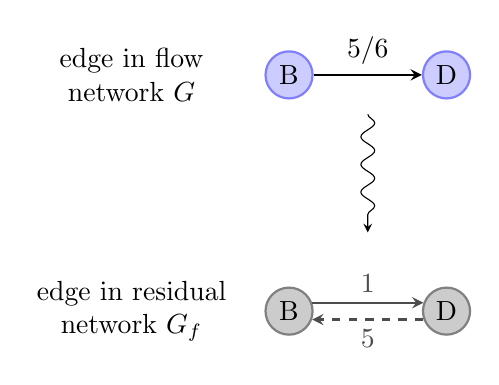
\begin{tikzpicture}
                [%x=10mm, y=9mm, 
                every text node part/.style={align=center},
                nsty/.style={circle, draw=blue!50, fill=blue!20, thick, inner sep=0.15em, minimum size=1.7em},
                rsty/.style={circle, draw=red!50, fill=red!20, thick, inner sep=0.15em, minimum size=1.7em},
                gsty/.style={circle, draw=black!50, fill=black!20, thick, inner sep=0.15em, minimum size=1.7em},
                asty/.style={-{stealth}, thick}]
                % flow network
                \node at (0,3) {edge in flow \\network \(G\)};
                \visible<1->{\node[nsty] (b) at (2,3) {B};}
                \visible<1->{\node[nsty] (d) at (4,3) {D};}
                \visible<1->{\draw[asty] (b) -- node[auto]{5/6} (d);}
                % transition
                \visible<2->{\draw[-{stealth}, snake=snake, line after snake=1mm] (3,2.5) -- (3,1);}
                % residual network
                \visible<2->{\node at (0,0) {edge in residual \\network \(G_f\)};}
                \visible<2->{\node[gsty] (b') at (2,0) {B};}
                \visible<2->{\node[gsty] (d') at (4,0) {D};}  
                \visible<2->{\draw[asty, black!70] (b'.20) -- node[auto]{1} (d'.160);}
                \visible<2->{\draw[asty, dashed, black!70] (d'.-160) -- node[auto]{5} (b'.-20);}
            \end{tikzpicture}
        \end{column}
        \begin{column}<3->{0.55\linewidth}
            \begin{definition}[Residual Network]
                \visible<4->{
                A {\color{red}residual network} of \(G\) induced by \(f\) is \(G_f=(V, E_f)\) with
                \begin{equation*}
                    E_f=\{(u,v)\in V\times V\mid c_f(u,v)>0\},
                \end{equation*}
                where} the {\color{black!70}\color<3->{red}residual capacity \(c_f\)} is given by
                \begin{equation*}
                    {\color{black!80}c_f(u,v)}=\left\{\begin{array}{ll} \!{\color{blue!70}c(u,v)-f(u,v)} & \!\text{if }(u,v)\in E \\ \!{\color{blue!70}f(v,u)} & \!\text{if }(v,u)\in E \\ \!0 & \!\text{otherwise} \end{array}\right.
                \end{equation*}
            \end{definition}
        \end{column}
    \end{columns}
\end{frame}

\subsection*{Demonstration of Ford-Fulkerson Method}
\begin{frame}
    \begin{columns}[c]
        \begin{column}<1->{0.5\linewidth}
            \begin{tikzpicture}
                [x=10mm, y=9mm, 
                nsty/.style={circle, draw=blue!50, fill=blue!20, thick, inner sep=0.15em, minimum size=1.7em},
                rsty/.style={circle, draw=red!50, fill=red!20, thick, inner sep=0.15em, minimum size=1.7em},
                asty/.style={-{stealth}, thick}]
                % nodes
                \visible<1->{\node[nsty] (s) at (-2,0) {s};}
                \visible<1->{\node[nsty] (a) at (0,2)  {A};}
                \visible<1->{\node[nsty] (b) at (0,-2) {B};}
                \visible<1->{\node[nsty] (c) at (2,2)  {C};}
                \visible<1->{\node[nsty] (d) at (2,-2) {D};}
                \visible<1->{\node[nsty] (t) at (4,0)  {t};}
                % max flow found
                \visible<1->{\draw[asty] (s) -- node[auto]                 {\only<2,22-23,32-34,51-52,57-59,63-66>{\color{red}}\only<2-22>{0}\only<23-51>{2}\only<52-63>{4}\only<64->{5}\color<2,22-23,32,51-52,63-64>{black}/6} (a);}
                \visible<1->{\draw[asty] (s) -- node[auto, swap]           {\only<2,8-12>{\color{red}}\only<2-7>{0}\only<8->{3}\color<2,8-10>{black}/3} (b);}
                \visible<1->{\draw[asty] (b) -- node[auto]                 {\only<2,8-10,13-14,53-54,57-59,63-66>{\color{red}}\only<2-7>{0}\only<8-53>{3}\only<54-63>{1}\only<64->{0}\color<2,8-10,53-54,63-64>{black}/7} (a);}
                \visible<1->{\draw[asty] (a) -- node[auto]                 {\only<2,8-10,15-16,24-25,32-37>{\color{red}}\only<2-7>{0}\only<8-24>{3}\only<25->{5}\color<2,8-10,24-25,32-34>{black}/5} (c);}
                \visible<1->{\draw[asty] (b) -- node[auto, swap]           {\only<2,28-29,32-42,55-59,63-66>{\color{red}}\only<2-28>{0}\only<29-55>{2}\only<56-63>{4}\only<64->{5}\color<2,28-29,32-40,55-56,63-64>{black}/6} (d);}
                \visible<1->{\draw[asty] (c) -- node[midway, sloped, above]{\only<2,26-27,32-40>{\color{red}}\only<2-26>{0}\only<27->{2}\color<2,26-27,32-37>{black}/2} (b);}
                \visible<1->{\draw[asty] (d) -- node[auto, swap]           {\only<2,63-66>{\color{red}}\only<2-63>{0}\only<64->{1}\color<2,63-64>{black}/3} (c);}
                \visible<1->{\draw[asty] (c) -- node[auto]                 {\only<2,8-10,17-18,63-66>{\color{red}}\only<2-7>{0}\only<8-63>{3}\only<64->{4}\color<2,8-10,63-64>{black}/7} (t);}
                \visible<1->{\draw[asty] (d) -- node[auto, swap]           {\only<2,30-44,55-59>{\color{red}}\only<2-30>{0}\only<31-55>{2}\only<56->{4}\color<2,30-42,55-56>{black}/4} (t);}
                % path 1 ab overlay 6
                % path 2 ab overlay 19
                % next up: update residual graph on 33
                % path 3 ab overlay 45
                % update residual graph on 58
                % path 4: overlay 60
                % termination 68
            \end{tikzpicture}
        \end{column}
        \begin{column}<3->{0.5\linewidth}
            \begin{tikzpicture}
                [x=10mm, y=9mm, 
                nsty/.style={circle, draw=blue!50, fill=blue!20, thick, inner sep=0.15em, minimum size=1.7em},
                rsty/.style={circle, draw=red!50, fill=red!20, thick, inner sep=0.15em, minimum size=1.7em},
                gsty/.style={circle, draw=black!50, fill=black!20, thick, inner sep=0.15em, minimum size=1.7em},
                %gsty/.style={circle, draw=green!50!black!50, fill=green!70!black!20, thick, inner sep=0.15em, minimum size=1.7em}, % green
                asty/.style={-{stealth}, thick}]
                % nodes
                \visible<3->{\node[gsty] (s) at (-2,0) {s};}
                \visible<3->{\node[gsty] (a) at (0,2)  {A};}
                \visible<3->{\node[gsty] (b) at (0,-2) {B};}
                \visible<3->{\node[gsty] (c) at (2,2)  {C};}
                \visible<3->{\node[gsty] (d) at (2,-2) {D};}
                \visible<3->{\node[gsty] (t) at (4,0)  {t};}
                % red
                \visible<6-8,20-31,46-56,61-64,68-69>{\node[rsty] at (-2,0) {s};}
                \visible<6-8,20-31,47-56,61-64,69>{\node[rsty] at (0,2)  {A};}
                \visible<6-8,20-31,48-56,61-64>{\node[rsty] at (0,-2) {B};}
                \visible<6-8,20-31,61-64>{\node[rsty] at (2,2)  {C};}
                \visible<30,20-31,49-56,61-64>{\node[rsty] at (2,-2) {D};}
                \visible<6-8,20-31,49-56,61-64>{\node[rsty] at (4,0)  {t};}

                % residual edges forward
                \visible<3->{\draw[asty] (s.60)   -- node[auto, outer sep=-3pt]                   {\only<34,58-59,66>{\color{red}}\only<3-33>{6}\only<34-57>{4}\only<58-65>{2}\only<66->{1}} (a.-150);}
                \visible<3-10>{\draw[asty] (s.-30)  -- node[auto, outer sep=-3pt]                   {\only<7-8>{\color{red}}\only<3-10>{3}} (b.120);}
                \visible<3->{\draw[asty] (b.105)  -- node[auto, outer sep=-1.5pt]                 {\only<14,58-59,66>{\color{red}}\only<3-13>{7}\only<14-57>{4}\only<58-65>{6}\only<66->{7}} (a.-105);}
                \visible<3-35>{\draw[asty] (a.15)   -- node[auto, outer sep=-1.5pt]                 {\only<16,21-31>{\color{red}}\only<3-15>{5}\only<16->{2}} (c.165);}
                \visible<3->{\draw[asty] (b.15)   -- node[auto, outer sep=-1.5pt]                 {\only<42,58-59,66>{\color{red}}\only<3-41>{6}\only<42-57>{4}\only<58-65>{2}\only<66->{1}} (d.165);}
                \visible<3-38>{\draw[asty] (c.-150) -- node[midway, sloped, above, outer sep=-1.5pt]{\only<21-31>{\color{red}}\only<3->{2}} (b.60);}
                \visible<3->{\draw[asty] (d.105)  -- node[auto, outer sep=-1.5pt]                 {\only<66>{\color{red}}\only<3-65>{3}\only<66->{2}} (c.-105);}
                \visible<3->{\draw[asty] (c.-30)  -- node[auto, outer sep=-3pt]                   {\only<18,66>{\color{red}}\only<3-17>{7}\only<18-65>{4}\only<66>{3}} (t.120);}
                \visible<3-57>{\draw[asty] (d.60)   -- node[auto, outer sep=-3pt]                   {\only<44,50-56,58-59>{\color{red}}\only<3-43>{4}\only<44-57>{2}} (t.-150);}
                \only<20-31,47-56,61-64,69>{\draw[asty, red, line width=0.4mm] (s.60)   to (a.-150);}
                \only<6-8>{\draw[asty, red, line width=0.4mm] (s.-30)  to (b.120);}
                \only<6-8>{\draw[asty, red, line width=0.4mm] (b.105)  to (a.-105);}
                \only<6-8,20-31>{\draw[asty, red, line width=0.4mm] (a.15)   to (c.165);}
                \only<20-31,49-56,61-64>{\draw[asty, red, line width=0.4mm] (b.15)   to (d.165);}
                \only<20-31>{\draw[asty, red, line width=0.4mm] (c.-150) to (b.60);}
                \only<61-64>{\draw[asty, red, line width=0.4mm] (d.105)  to (c.-105);}
                \only<6-8,61-64>{\draw[asty, red, line width=0.4mm] (c.-30)  to (t.120);}
                \only<20-31,49-56>{\draw[asty, red, line width=0.4mm] (d.60)   to (t.-150);}
                % residual edges forward 0
                \visible<11>{\draw[asty, black!30] (s.-30)  -- node[auto, outer sep=-3pt]{0} (b.120);}
                \visible<36>{\draw[asty, black!30] (a.15)   -- node[auto, outer sep=-1.5pt]{0} (c.165);}
                \visible<39>{\draw[asty, black!30] (c.-150) -- node[midway, sloped, above, outer sep=-1.5pt]{0} (b.60);}
                \visible<58>{\draw[asty, black!30] (d.60)   -- node[auto, outer sep=-3pt]{0} (t.-150);}
                
                % residual edges backward 0
                \visible<4>{\draw[asty, dashed, black!30] (a.-120) -- node[auto, outer sep=-3pt]  {0} (s.30);}
                \visible<4>{\draw[asty, dashed, black!30] (b.150)  -- node[auto, outer sep=-3pt]  {0} (s.-60);}
                \visible<4,66>{\draw[asty, dashed, black!30] (a.-75)  -- node[auto, outer sep=-1.5pt]{0} (b.75);}
                \visible<4>{\draw[asty, dashed, black!30] (c.-165) -- node[auto, outer sep=-1.5pt]{0} (a.-15);}
                \visible<4>{\draw[asty, dashed, black!30] (d.-165) -- node[auto, outer sep=-1.5pt]{0} (b.-15);}
                \visible<4>{\draw[asty, dashed, black!30] (b.30)   -- node[midway, sloped, below, outer sep=-1.5pt]{0} (c.-120);}
                \visible<4>{\draw[asty, dashed, black!30] (c.-75)  -- node[auto, outer sep=-1.5pt]{0} (d.75);}
                \visible<4>{\draw[asty, dashed, black!30] (t.150)  -- node[auto, outer sep=-3pt]  {0} (c.-60);}
                \visible<4>{\draw[asty, dashed, black!30] (t.-120) -- node[auto, outer sep=-3pt]  {0} (d.30);}
                % residual edges backward
                \visible<34->{\draw[asty, dashed, black!70] (a.-120) -- node[auto, outer sep=-3pt]                   {\only<34,58-59,66>{\color{red}}\only<34-57>{2}\only<58-65>{4}\only<66->{5}} (s.30);}
                \visible<10->{\draw[asty, dashed, black!70] (b.150)  -- node[auto, outer sep=-3pt]                   {\only<10>{\color{red}}\only<9->{3}} (s.-60);}
                \visible<10-65>{\draw[asty, dashed, black!70] (a.-75)  -- node[auto, outer sep=-1.5pt]                 {\only<10,58-59,62-64,66>{\color{red}}\only<9-57>{3}\only<58-65>{1}} (b.75);}
                \visible<10->{\draw[asty, dashed, black!70] (c.-165) -- node[auto, outer sep=-1.5pt]                 {\only<10,36-37>{\color{red}}\only<9-35>{3}\only<36->{5}} (a.-15);}
                \visible<42->{\draw[asty, dashed, black!70] (d.-165) -- node[auto, outer sep=-1.5pt]                 {\only<42,58-59,66>{\color{red}}\only<42-57>{2}\only<58-65>{4}\only<66->{5}} (b.-15);}
                \visible<39->{\draw[asty, dashed, black!70] (b.30)   -- node[midway, sloped, below, outer sep=-1.5pt]{\only<39-40>{\color{red}}\only<39->{2}} (c.-120);}
                \visible<66->{\draw[asty, dashed, black!70] (c.-75)  -- node[auto, outer sep=-1.5pt]                 {\only<66>{\color{red}}\only<66->{1}} (d.75);}
                \visible<10->{\draw[asty, dashed, black!70] (t.150)  -- node[auto, outer sep=-3pt]                   {\only<10,66>{\color{red}}\only<9-65>{3}\only<66->{4}} (c.-60);}
                \visible<44->{\draw[asty, dashed, black!70] (t.-120) -- node[auto, outer sep=-3pt]                   {\only<44,58-59>{\color{red}}\only<44-57>{2}\only<58->{4}} (d.30);}
                \visible<48-56,61-64>{\draw[asty, dashed, red, line width=0.4mm] (a.-75) to (b.75);}
                %%\visible<1->{\draw[asty, dashed,black!70] (c) [out=135, in=45] to node[auto]{\only<2>{0/0}\only<3->{0/5}} (a);}
            \end{tikzpicture}
        \end{column}
    \end{columns}
\end{frame}

\subsection*{Correctness of Ford-Fulkerson Method}
\begin{frame}{\(\ \)}
    \centering
    \begin{tikzpicture}
        [x=10mm, y=9mm,
        every text node part/.style={align=center},
        nsty/.style={circle, draw=blue!50, fill=blue!20, thick, inner sep=0.15em, minimum size=1.7em},
        rsty/.style={circle, draw=red!50, fill=red!20, thick, inner sep=0.15em, minimum size=1.7em},
        asty/.style={-{stealth}, thick}]
        \begin{scope}[on background layer]
            %\visible<2-3>{\draw [draw=orange!20, fill=orange!20] (-2.5,0.7) -- (-2.5,-0.7) -- (-0.6,-2.55) -- (0.4,-2.55) -- (0.4, 2.55) -- (-0.6,2.55) -- cycle;}
            %\visible<2-3>{\draw [draw=orange!20, fill=orange!20] (4.5,0.7) -- (4.5,-0.7) -- (2.6,-2.55) -- (1.6,-2.55) -- (1.6, 2.55) -- (2.6,2.55) -- cycle;}
            %\node [fill=black!30, fit= (s) (a) (b)]{};
            %\node [fill=black!30, ellipse, fit= (t) (c) (d)]{};
            \visible<2>{\draw[draw=orange!20, fill=orange!20] plot [smooth cycle] coordinates {(-2.5,0.7)(-2.5,-0.7)(-0.6,-2.55)(0.4,-2.55)(0.4, 2.55)(-0.6,2.55)};}
            \visible<2>{\draw[draw=orange!20, fill=orange!20] plot [smooth cycle] coordinates {(4.5,0.7)(4.5,-0.7)(2.6,-2.55)(1.6,-2.55)(1.6, 2.55)(2.6,2.55)};}
            \visible<3->{\draw [draw=orange!20, fill=orange!20] plot[smooth cycle] coordinates {(-2.5,0.7)(-2.5,-0.5)(-1.5,-1)(0.45,1.8)(0.5, 2.5)(-0.7,2.5)};}
            \visible<3->{\draw [draw=orange!20, fill=orange!20] plot[smooth cycle] coordinates {(4.5,0.7)(4.5,-0.7)(2.6,-2.55)(-0.6,-2.55)(-0.6,-1.45)(1.6, 2.55)(2.6,2.55)};}
        \end{scope}
        \clip (-5.1,-2.7) rectangle (7.1,2.7); 
        % nodes
        \node[nsty] (s) at (-2,0) {s};
        \node[nsty] (a) at (0,2)  {A};
        \node[nsty] (b) at (0,-2) {B};
        \node[nsty] (c) at (2,2)  {C};
        \node[nsty] (d) at (2,-2) {D};
        \node[nsty] (t) at (4,0)  {t};
        \node at (-4,0) {value of flow:\\\(8 = {\color<4->{red}5}+{\color<4->{blue!80}3}\)};
        % verticies and flow
        \draw[asty] (s) -- node[auto]      {{\color<4->{red}5}/6} (a);
        \draw[asty] (s) -- node[auto, swap]{{\color<4->{blue!80}3}/{\color<4->{green!60!black!100}3}} (b);
        \draw[asty] (b) -- node[auto]      {0/7} (a);
        \draw[asty] (a) -- node[auto]      {{\color<4->{blue!80}5}/{\color<4->{green!60!black!100}5}} (c);
        \draw[asty] (b) -- node[auto, swap]{5/6} (d);
        \draw[asty] (c) -- node[midway, sloped, above]{2/2} (b);
        \draw[asty] (d) -- node[auto, swap]{1/3} (c);
        \draw[asty] (c) -- node[auto]      {4/7} (t);
        \draw[asty] (d) -- node[auto, swap]{4/4} (t);
    \end{tikzpicture}
    \vspace*{-5mm}
    \visible<2->{
    \begin{align*}
        \text{net flow across cut: }\only<2>{\ 8 &=5-2+5}\only<3>{\qquad\qquad}\only<4->{8 &={\color<4->{blue!80}5}+{\color<4->{blue!80}3}} \\
        \text{capacity of cut: }\only<2>{11 &= 5+6}\only<3>{\qquad\qquad}\only<4->{8 &={\color<4->{green!60!black!100}5}+{\color<4->{green!60!black!100}3}}
    \end{align*}}
\end{frame}

\begin{frame}{Partial Correctness\only<2>{ and Termination}}
    \begin{columns}[c]
        \only<1->{
            \begin{column}{0.45\textwidth}
                \begin{block}{Max-Flow Min-Cut Theorem}
                    For a flow \(f\) in \(G=(V,E)\) the following conditions are equivalent
                    \begin{enumerate}
                        \item \(f\) is a maximum flow
                        \item there is no augmenting path in \(G_f\)
                        \item the value of flow equals capacity of some cut of \(G\)
                    \end{enumerate}
                \end{block}
                \vspace*{3mm}
                \visible<2->{Termination: 

                in each iteration the flow is increased by at least one unit}
                \vspace*{8mm}
            \end{column}
        }
        \begin{column}<1->{0.55\linewidth}
            \centering \vspace*{-3mm}

            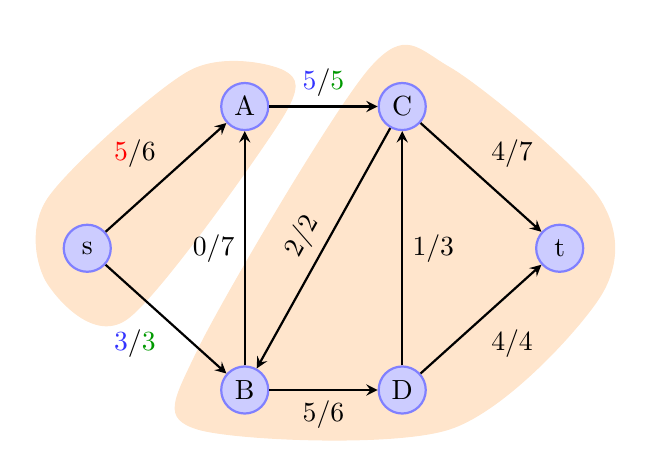
\begin{tikzpicture}
                [x=10mm, y=9mm,
                nsty/.style={circle, draw=blue!50, fill=blue!20, thick, inner sep=0.15em, minimum size=1.7em},
                asty/.style={-{stealth}, thick}]
                % nodes
                \node[nsty] (s) at (-2,0) {s};
                \node[nsty] (a) at (0,2)  {A};
                \node[nsty] (b) at (0,-2) {B};
                \node[nsty] (c) at (2,2)  {C};
                \node[nsty] (d) at (2,-2) {D};
                \node[nsty] (t) at (4,0)  {t};
                % verticies and flow
                \draw[asty] (s) -- node[auto]      {{\color{red}5}/6} (a);
                \draw[asty] (s) -- node[auto, swap]{{\color{blue!80}3}/{\color{green!60!black!100}3}} (b);
                \draw[asty] (b) -- node[auto]      {0/7} (a);
                \draw[asty] (a) -- node[auto]      {{\color{blue!80}5}/{\color{green!60!black!100}5}} (c);
                \draw[asty] (b) -- node[auto, swap]{5/6} (d);
                \draw[asty] (c) -- node[midway, sloped, above]{2/2} (b);
                \draw[asty] (d) -- node[auto, swap]{1/3} (c);
                \draw[asty] (c) -- node[auto]      {4/7} (t);
                \draw[asty] (d) -- node[auto, swap]{4/4} (t);
                \begin{scope}[on background layer]
                    \draw [draw=orange!20, fill=orange!20] plot[smooth cycle] coordinates {(-2.5,0.7)(-2.5,-0.5)(-1.5,-1)(0.45,1.8)(0.5, 2.5)(-0.7,2.5)};
                    \draw [draw=orange!20, fill=orange!20] plot[smooth cycle] coordinates {(4.5,0.7)(4.5,-0.7)(2.6,-2.55)(-0.6,-2.55)(-0.6,-1.45)(1.6, 2.55)(2.6,2.55)};
                    %\draw [draw=orange!20, fill=orange!20] (-2.5,0.7) -- (-2.5,-0.5) -- (-1.5,-1) -- (0.45,1.8) -- (0.5, 2.5) -- (-0.7,2.5) -- cycle;
                    %\draw [draw=orange!20, fill=orange!20] (4.5,0.7) -- (4.5,-0.7) -- (2.6,-2.55) -- (-0.6,-2.55) -- (-0.6,-1.45) -- (1.6, 2.55) -- (2.6,2.55) -- cycle;
                \end{scope}
            \end{tikzpicture}
            \vspace*{-5mm}
            \only<1->{
            \begin{align*}
                \text{value of flow: }8 &= {\color{red}5}+{\color{blue!80}3}\\
                \text{net flow across cut: }8 &={\color{blue!80}5}+{\color{blue!80}3} \\
                \text{capacity of cut: }8 &={\color{green!60!black!100}5}+{\color{green!60!black!100}3}
            \end{align*}}
        \end{column}
    \end{columns}
\end{frame}

\subsection*{Analysis of Time Complexity of Ford-Fulkerson Method}
\begin{frame}{Time Complexity}
    \begin{columns}[c]
        \begin{column}<1->{0.65\linewidth}
            
            \begin{itemize}[<+->]
                \item method to find augmenting paths unspecified in Ford-Fulkerson Method
                \item use e.g. Depth-First Search (DFS) for finding augmenting paths (i.e. random choice), takes \(O(\lvert V \rvert + 2\lvert E \rvert)=O(\lvert E\rvert)\) time
                \item initializing and updating residual network takes \(O(\lvert E\rvert)\) time as well
                \item maximum number of iterations: \color{red}value of flow \(\lvert f\rvert\)
                \item[\(\Rightarrow\)] \(\lvert f\rvert\) iterations of \(O(\lvert E\rvert)\) yields \(O({\color{red}\lvert f\rvert}\cdot \lvert E\rvert)\) in total
            \end{itemize}
        \end{column}
        \begin{column}<4->{0.35\linewidth}
            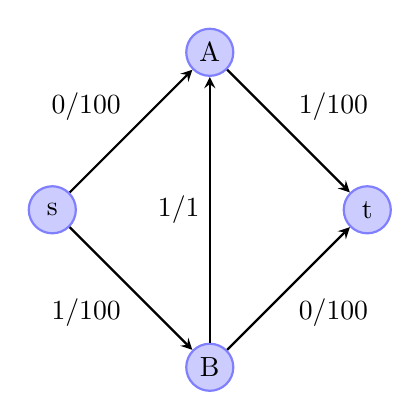
\begin{tikzpicture}
                [x=10mm, y=10mm, 
                nsty/.style={circle, draw=blue!50, fill=blue!20, thick, inner sep=0.15em, minimum size=1.7em},
                rsty/.style={circle, draw=red!50, fill=red!20, thick, inner sep=0.15em, minimum size=1.7em},
                asty/.style={-{stealth}, thick}]
                % nodes
                \node[nsty] (s) at (-2,0) {s};
                \node[nsty] (a) at (0,2)  {A};
                \node[nsty] (b) at (0,-2) {B};
                \node[nsty] (t) at (2,0)  {t};
                % vertices
                \draw[asty] (s) -- node[auto]      {0/100} (a);
                \draw[asty] (s) -- node[auto, swap]{1/100} (b);
                \draw[asty] (b) -- node[auto]      {1/1} (a);
                \draw[asty] (a) -- node[auto]      {1/100} (t);
                \draw[asty] (b) -- node[auto, swap]{0/100} (t);
            \end{tikzpicture}
        \end{column}
    \end{columns}
\end{frame}


\section{Optimizations of Ford-Fulkerson Method}
\begin{frame}{Optimizing Ford-Fulkerson Method}
    Idea: vary method of finding augmenting paths by
    \begin{itemize}
        \item doing Breadth-First Search (BFS)
        \item choosing paths of high bottle neck value first
        \item using so-called level graph to find shortest augmenting paths 
    \end{itemize}
\end{frame}

\subsection*{Edmonds-Karp Algorithm}
\begin{frame}{Edmonds-Karp Algorithm}
    \begin{columns}[c]
        \begin{column}<1->{0.65\linewidth}
            \begin{itemize}
                \item use BFS to find augmenting paths
                \item shortest-path distance increases monotonically with flow augmentation
                \item maximum number of iterations: \(O(VE)\)
                \begin{itemize}
                    \item maximum number of augmenting paths of same length: \(\lvert E\rvert\)
                    \item maximum length of any path: \(\lvert V\rvert\)
                \end{itemize}
                \item in total: \(O(VE^2)\) which is independent of maximum flow value
            \end{itemize}
        \end{column}
        \begin{column}<1->{0.35\linewidth}
            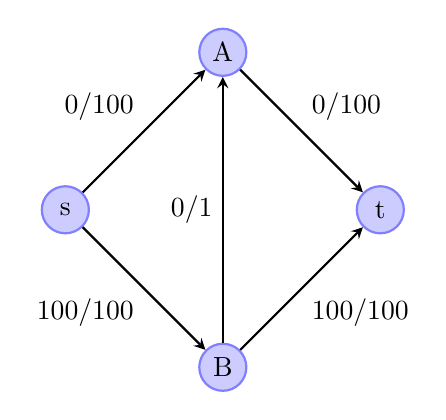
\begin{tikzpicture}
                [x=10mm, y=10mm, 
                nsty/.style={circle, draw=blue!50, fill=blue!20, thick, inner sep=0.15em, minimum size=1.7em},
                rsty/.style={circle, draw=red!50, fill=red!20, thick, inner sep=0.15em, minimum size=1.7em},
                asty/.style={-{stealth}, thick}]
                % nodes
                \node[nsty] (s) at (-2,0) {s};
                \node[nsty] (a) at (0,2)  {A};
                \node[nsty] (b) at (0,-2) {B};
                \node[nsty] (t) at (2,0)  {t};
                % vertices
                \draw[asty] (s) -- node[auto]      {0/100} (a);
                \draw[asty] (s) -- node[auto, swap]{100/100} (b);
                \draw[asty] (b) -- node[auto]      {0/1} (a);
                \draw[asty] (a) -- node[auto]      {0/100} (t);
                \draw[asty] (b) -- node[auto, swap]{100/100} (t);
            \end{tikzpicture}
        \end{column}
    \end{columns}
\end{frame}

\subsection*{Capacity Scaling}
\begin{frame}{Capacity Scaling}
    \begin{columns}[c]
        \begin{column}<1->{0.5\linewidth}
            \begin{itemize}[<+->]
                \item heuristic to choose paths of high capacity first
                \item \color<9>{red}highest capacity of all edges \(C_{max}\)
                \item lower capacity bound \(\Delta\)
                \item \color<10>{red}start with \(\Delta = 2^n \leq C_{max} < 2^{n+1}\)
                \item \color<11-12,15-16>{red}only consider edges with capacities greater than or equal \(\Delta\) to find paths
                \item \color<14,18>{red}decrease \(\Delta\) if {\color<13,17>{red}there are no more paths}:\\\(\qquad\qquad\qquad\Delta\leftarrow \Delta/2\)
            \end{itemize}
        \end{column}
        \begin{column}<1->{0.5\linewidth}
            \begin{tikzpicture}
                [x=10mm, y=9mm, 
                nsty/.style={circle, draw=blue!50, fill=blue!20, thick, inner sep=0.15em, minimum size=1.7em},
                rsty/.style={circle, draw=red!50, fill=red!20, thick, inner sep=0.15em, minimum size=1.7em},
                gsty/.style={circle, draw=black!50, fill=black!20, thick, inner sep=0.15em, minimum size=1.7em},
                %gsty/.style={circle, draw=green!50!black!50, fill=green!70!black!20, thick, inner sep=0.15em, minimum size=1.7em}, % green
                asty/.style={-{stealth}, thick}]
                %%%%%%%%%%%%% flow graph %%%%%%%%%%%%%%%%%%%
                % nodes
                \visible<7>{\node[nsty] (s) at (-2,0) {s};}
                \visible<7>{\node[nsty] (a) at (0,2)  {A};}
                \visible<7>{\node[nsty] (b) at (0,-2) {B};}
                \visible<7>{\node[nsty] (c) at (2,2)  {C};}
                \visible<7>{\node[nsty] (d) at (2,-2) {D};}
                \visible<7>{\node[nsty] (t) at (4,0)  {t};}
                % verticies and flow
                \visible<7>{\draw[asty] (s) -- node[auto]      {\only<7->{0}\only<8->{5}/6} (a);}
                \visible<7>{\draw[asty] (s) -- node[auto, swap]{0/3} (b);}
                \visible<7>{\draw[asty] (b) -- node[auto]      {0/7} (a);}
                \visible<7>{\draw[asty] (a) -- node[auto]      {0/5} (c);}
                \visible<7>{\draw[asty] (b) -- node[auto, swap]{0/6} (d);}
                \visible<7>{\draw[asty] (c) -- node[midway, sloped, above]{0/2} (b);}
                \visible<7>{\draw[asty] (d) -- node[auto, swap]{0/3} (c);}
                \visible<7>{\draw[asty] (c) -- node[auto]      {0/7} (t);}
                \visible<7>{\draw[asty] (d) -- node[auto, swap]{0/4} (t);}

                %%%%%%%%%%%%% residual graph %%%%%%%%%%%%%%%
                % nodes
                \visible<8->{\node[gsty] at (-2,0) {s};}
                \visible<8->{\node[gsty] at (0,2)  {A};}
                \visible<8->{\node[gsty] at (0,-2) {B};}
                \visible<8->{\node[gsty] at (2,2)  {C};}
                \visible<8->{\node[gsty] at (2,-2) {D};}
                \visible<8->{\node[gsty] at (4,0)  {t};}
                % red
                \visible<12,16,19>{\node[rsty] at (-2,0) {s};}
                \visible<12,19>{\node[rsty] at (0,2)  {A};}
                \visible<16>{\node[rsty] at (0,-2) {B};}
                \visible<12>{\node[rsty] at (2,2)  {C};}
                \visible<16>{\node[rsty] at (2,-2) {D};}
                \visible<12,16>{\node[rsty] at (4,0)  {t};}

                % residual edges forward
                \visible<8-12,18->{\draw[asty] (s.60)   -- node[auto, outer sep=-3pt]                   {\only<8-12>{6}\only<13->{1}} (a.-150);}
                \visible<8-10,15-16>{\draw[asty] (s.-30)  -- node[auto, outer sep=-3pt]                   {3} (b.120);}
                \visible<8->{\draw[asty] (b.105)  -- node[auto, outer sep=-1.5pt]                 {\color<9>{red}7} (a.-105);}
                \visible<8-12>{\draw[asty] (a.15)   -- node[auto, outer sep=-1.5pt]                 {5} (c.165);}
                \visible<8->{\draw[asty] (b.15)   -- node[auto, outer sep=-1.5pt]                 {\only<8-16>{6}\only<17->{3}} (d.165);}
                \visible<8-10,15->{\draw[asty] (c.-150) -- node[midway, sloped, above, outer sep=-1.5pt]{2} (b.60);}
                \visible<8-10,15->{\draw[asty] (d.105)  -- node[auto, outer sep=-1.5pt]                 {3} (c.-105);}
                \visible<8-12,15->{\draw[asty] (c.-30)  -- node[auto, outer sep=-3pt]                   {\color<9>{red}\only<8-12>{7}\only<13->{2}} (t.120);}
                \visible<8->{\draw[asty] (d.60)   -- node[auto, outer sep=-3pt]                   {\only<8-16>{4}\only<17->{1}} (t.-150);}
                % red
                \only<12,19>{\draw[asty, red, line width=0.4mm] (s.60)   to (a.-150);}
                \only<16>{\draw[asty, red, line width=0.4mm] (s.-30)  to (b.120);}
                \only<12>{\draw[asty, red, line width=0.4mm] (a.15)   to (c.165);}
                \only<16>{\draw[asty, red, line width=0.4mm] (b.15)   to (d.165);}
                \only<12>{\draw[asty, red, line width=0.4mm] (c.-30)  to (t.120);}
                \only<16>{\draw[asty, red, line width=0.4mm] (d.60)   to (t.-150);}
                % residual edges forward < Delta
                \only<13-17>{\draw[asty, black!20] (s.60)   -- node[auto, outer sep=-3pt]                   {1} (a.-150);}
                \only<11-14>{\draw[asty, black!20] (s.-30)  -- node[auto, outer sep=-3pt]                   {3} (b.120);}
                \only<11-14>{\draw[asty, black!20] (c.-150) -- node[midway, sloped, above, outer sep=-1.5pt]{2} (b.60);}
                \only<11-14>{\draw[asty, black!20] (d.105)  -- node[auto, outer sep=-1.5pt]                 {3} (c.-105);}
                \only<13-14>{\draw[asty, black!20] (c.-30)  -- node[auto, outer sep=-3pt]                   {2} (t.120);}
                
                % residual edges backward
                \visible<13->{\draw[asty, dashed] (a.-120) -- node[auto, outer sep=-3pt]                   {\only<13->{5}} (s.30);}
                \visible<17->{\draw[asty, dashed] (b.150)  -- node[auto, outer sep=-3pt]                   {3} (s.-60);}
                \visible<13->{\draw[asty, dashed] (c.-165) -- node[auto, outer sep=-1.5pt]                 {\only<13->{5}} (a.-15);}
                \visible<17->{\draw[asty, dashed] (d.-165) -- node[auto, outer sep=-1.5pt]                 {3} (b.-15);}
                \visible<13->{\draw[asty, dashed] (t.150)  -- node[auto, outer sep=-3pt]                   {\only<13->{5}} (c.-60);}
                \visible<17->{\draw[asty, dashed] (t.-120) -- node[auto, outer sep=-3pt]                   {3} (d.30);}
                
                % text nodes
                \node at (1,-3) {\color<10,14,18>{red}\(\visible<10->{\Delta=}\only<10-13>{4}\only<10>{=2^2\leq C_{max}<2^3}\only<14-17>{2}\only<14>{=4/2}\only<18->{1}\only<18>{=2/2}\)};
                \node at (1,-3.6) {\(\color<9>{red}\visible<9-10>{C_{max}=7}\)};
            \end{tikzpicture}
        \end{column}
    \end{columns}
\end{frame}

\begin{frame}{Time Complexity of Capacity Scaling}
    \begin{columns}[c]
        \begin{column}{0.86\textwidth}
            \vspace*{-5mm}
            \begin{block}{Ford-Fulkerson Method (with BFS) / Edmonds-Karp Algorithm}
                \begin{algorithmic}[1]
                    \STATE \(C_{max}\gets\) max capacity edge\tikzmark{cmax}; \(\Delta\gets 2^{\lfloor\log_2(C_{max})\rfloor}\)
                    \STATE initialize flow \(f\) with 0\tikzmark{init}
                    \WHILE{\(\Delta\geq 1\)\tikzmark{outerwhile}}
                    \STATE \(G_f(\Delta)\gets\) residual graph with edges of capacity \(\geq\Delta\)\tikzmark{gfd}
                    \WHILE{\tikzmark{while0}there exists an augmenting path\tikzmark{path} \(p\) in \(G_f(\Delta)\)\tikzmark{while}}
                    \STATE augment flow \(f\) along \(p\)\tikzmark{augment} and update \(G_f(\Delta)\)\tikzmark{update}
                    \ENDWHILE \tikzmark{while1}
                    \STATE \(\Delta\gets\Delta/2\)
                    \ENDWHILE
                    \RETURN \(f\)
                \end{algorithmic}
            \end{block}
        \end{column}
    \end{columns}
    %\AddTextShift{cmax}{\(O(E)\)}{red}{(0,-0.03)}
    %\AddTextShift{init}{\(O(E)\)}{blue!80}{(0,-0.03)}
    %\AddBraceTopShift{cmax}{init}{\(O(E)\)}{blue!80}{(1,0)}
    \AddTextShift{outerwhile}{\(O(\log(C_{max}))\) iterations}{red}{(0.5,-0.03)}
    %\AddTextShift{gfd}{\(O(E)\)}{red}{(0,-0.03)}
    %\AddArrowSouth{path}{BFS/DFS: \color{blue!80}\(O(E)\)}{blue!80}{(1.5,-1.3)}
    %\AddTextShift{augment}{\(O(E)\)}{blue!80}{(0,-0.03)}
    %\AddTextShift{update}{\(O(E)\)}{red}{(0,-0.03)}
    
    \centering DFS: \(O(E^2\log(C_{max}))\qquad\)BFS: \(O(EV\log(C_{max}))\)
\end{frame}

\subsection*{Dinic's Algorithm}
\begin{frame}{Dinic's Algorithm}
    \begin{columns}[c]
        \begin{column}{0.8\textwidth}
            \begin{itemize}
                \item uses shortest augmenting paths (like Edmonds-Karp Algorithm)
                \item find augmenting flows in level graph created from BFS
                \item time complexity: \(O(V^2E)\)
            \end{itemize}
            \begin{block}<1->{Dinic's Algorithm}
                \begin{algorithmic}
                    \STATE initialize flow \(f\) with 0
                    \WHILE{there exists an s-t-path in the residual network \(G_f\)}
                    \STATE \(G_L\gets\) {\color{red}level graph} from BFS on \(G_f\)
                    \STATE find {\color{red}blocking flow} \(f'\) in \(G_L\) by DFS
                    \STATE augment flow \(f\) by \(f'\)
                    \ENDWHILE
                    \RETURN \(f\)
                \end{algorithmic}
            \end{block}
        \end{column}
    \end{columns}
\end{frame}

\begin{frame}
    \begin{definition}[Level Graph]
        The {\color{red}level graph} of a residual network \(G_f=(V, E_f)\) is a graph \(G_L=(V, E_L)\) with 
        \begin{equation*}
            E_L=\{(u,v)\in E_f\mid \operatorname*{dist}(v) = \operatorname*{dist}(u)+1\}
        \end{equation*}
    \end{definition}
    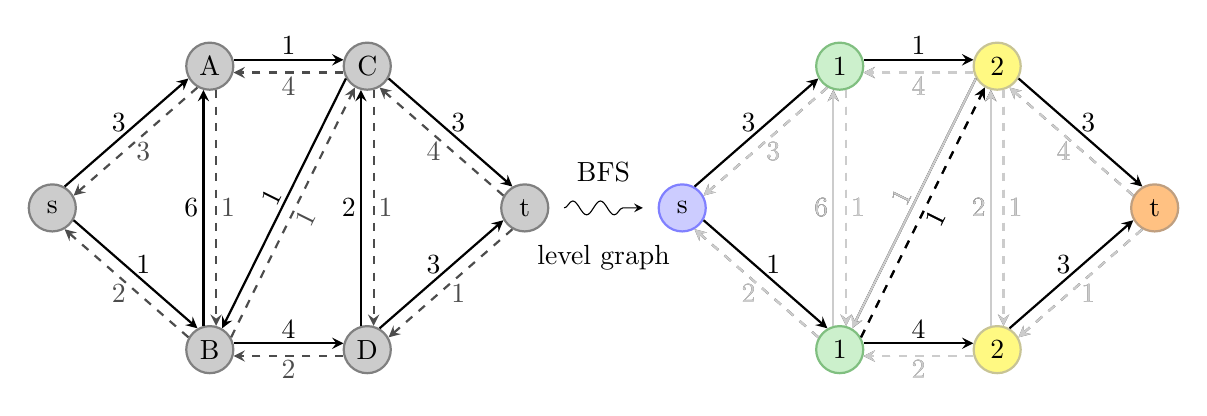
\begin{tikzpicture}
        [x=10mm, y=9mm, 
        nsty/.style={circle, draw=blue!50, fill=blue!20, thick, inner sep=0.15em, minimum size=1.7em},
        rsty/.style={circle, draw=red!50, fill=red!20, thick, inner sep=0.15em, minimum size=1.7em},
        ysty/.style={circle, draw=yellow!50!black!50, fill=yellow!70!white!70, thick, inner sep=0.15em, minimum size=1.7em},
        osty/.style={circle, draw=orange!50!black!50, fill=orange!70!white!70, thick, inner sep=0.15em, minimum size=1.7em},
        gsty/.style={circle, draw=black!50, fill=black!20, thick, inner sep=0.15em, minimum size=1.7em},
        grsty/.style={circle, draw=green!50!black!50, fill=green!70!black!20, thick, inner sep=0.15em, minimum size=1.7em}, % green
        asty/.style={-{stealth}, thick}]
        %%%%%%%%%%% first graph %%%%%%%%%%%%%%%%%%%%
        \visible<2->{\node[gsty] (s) at (-2,0) {s};}
        \visible<2->{\node[gsty] (a) at (0,2)  {A};}
        \visible<2->{\node[gsty] (b) at (0,-2) {B};}
        \visible<2->{\node[gsty] (c) at (2,2)  {C};}
        \visible<2->{\node[gsty] (d) at (2,-2) {D};}
        \visible<2->{\node[gsty] (t) at (4,0)  {t};}
        
        %% residual edges forward
        \visible<2->{\draw[asty] (s.60)   -- node[auto, outer sep=-3pt]                   {3} (a.-150);}
        \visible<2->{\draw[asty] (s.-30)  -- node[auto, outer sep=-3pt]                   {1} (b.120);}
        \visible<2->{\draw[asty] (b.105)  -- node[auto, outer sep=-1.5pt]                 {6} (a.-105);}
        \visible<2->{\draw[asty] (a.15)   -- node[auto, outer sep=-1.5pt]                 {1} (c.165);}
        \visible<2->{\draw[asty] (b.15)   -- node[auto, outer sep=-1.5pt]                 {4} (d.165);}
        \visible<2->{\draw[asty] (c.-150) -- node[midway, sloped, above, outer sep=-1.5pt]{1} (b.60);}
        \visible<2->{\draw[asty] (d.105)  -- node[auto, outer sep=-1.5pt]                 {2} (c.-105);}
        \visible<2->{\draw[asty] (c.-30)  -- node[auto, outer sep=-3pt]                   {3} (t.120);}
        \visible<2->{\draw[asty] (d.60)   -- node[auto, outer sep=-3pt]                   {3} (t.-150);}
        
        % residual edges backward
        \visible<2->{\draw[asty, dashed, black!70] (a.-120) -- node[auto, outer sep=-3pt]  {3} (s.30);}
        \visible<2->{\draw[asty, dashed, black!70] (b.150)  -- node[auto, outer sep=-3pt]  {2} (s.-60);}
        \visible<2->{\draw[asty, dashed, black!70] (a.-75)  -- node[auto, outer sep=-1.5pt]{1} (b.75);}
        \visible<2->{\draw[asty, dashed, black!70] (c.-165) -- node[auto, outer sep=-1.5pt]{4} (a.-15);}
        \visible<2->{\draw[asty, dashed, black!70] (b.30)   -- node[midway, sloped, below, outer sep=-1.5pt]{1} (c.-120);}
        \visible<2->{\draw[asty, dashed, black!70] (d.-165) -- node[auto, outer sep=-1.5pt]{2} (b.-15);}
        \visible<2->{\draw[asty, dashed, black!70] (c.-75)  -- node[auto, outer sep=-1.5pt]{1} (d.75);}
        \visible<2->{\draw[asty, dashed, black!70] (t.150)  -- node[auto, outer sep=-3pt]  {4} (c.-60);}
        \visible<2->{\draw[asty, dashed, black!70] (t.-120) -- node[auto, outer sep=-3pt]  {1} (d.30);}
        
        %%%%%%%%%%% transition %%%%%%%%%%%%%%%%%%%%%
        \visible<3->{\draw[-{stealth}, snake=snake, line after snake=1mm] (4.5,0) -- (5.5,0);}
        \visible<3->{\node at (5,0.5) {BFS};}
        \visible<4->{\node at (5,-0.7) {level graph};}
        
        %%%%%%%%%%% second graph %%%%%%%%%%%%%%%%%%%
        \visible<3-5>{\node[nsty] (s) at (6,0) {s};}
        \visible<3->{\node[grsty] (a) at (8,2)  {1};}
        \visible<3->{\node[grsty] (b) at (8,-2) {1};}
        \visible<3->{\node[ysty] (c) at (10,2)  {2};}
        \visible<3->{\node[ysty] (d) at (10,-2) {2};}
        \visible<3->{\node[osty] (t) at (12,0)  {t};}

        %% residual edges forward
        \visible<3->{\draw[asty] (s.60)   -- node[auto, outer sep=-3pt]                   {3} (a.-150);}
        \visible<3->{\draw[asty] (s.-30)  -- node[auto, outer sep=-3pt]                   {1} (b.120);}
        \visible<3>{\draw[asty] (b.105)  -- node[auto, outer sep=-1.5pt]                 {6} (a.-105);}
        \visible<3->{\draw[asty] (a.15)   -- node[auto, outer sep=-1.5pt]                 {1} (c.165);}
        \visible<3->{\draw[asty] (b.15)   -- node[auto, outer sep=-1.5pt]                 {4} (d.165);}
        \visible<3>{\draw[asty] (c.-150) -- node[midway, sloped, above, outer sep=-1.5pt]{1} (b.60);}
        \visible<3>{\draw[asty] (d.105)  -- node[auto, outer sep=-1.5pt]                 {2} (c.-105);}
        \visible<3->{\draw[asty] (c.-30)  -- node[auto, outer sep=-3pt]                   {3} (t.120);}
        \visible<3->{\draw[asty] (d.60)   -- node[auto, outer sep=-3pt]                   {3} (t.-150);}
        
        % residual edges backward
        \visible<3>{\draw[asty, dashed, black!70] (a.-120) -- node[auto, outer sep=-3pt]  {3} (s.30);}
        \visible<3>{\draw[asty, dashed, black!70] (b.150)  -- node[auto, outer sep=-3pt]  {2} (s.-60);}
        \visible<3>{\draw[asty, dashed, black!70] (a.-75)  -- node[auto, outer sep=-1.5pt]{1} (b.75);}
        \visible<3>{\draw[asty, dashed, black!70] (c.-165) -- node[auto, outer sep=-1.5pt]{4} (a.-15);}
        \visible<3>{\draw[asty, dashed, black!70] (b.30)   -- node[midway, sloped, below, outer sep=-1.5pt]{1} (c.-120);}
        \visible<4->{\draw[asty, dashed,        ] (b.30)   -- node[midway, sloped, below, outer sep=-1.5pt]{1} (c.-120);}
        \visible<3>{\draw[asty, dashed, black!70] (d.-165) -- node[auto, outer sep=-1.5pt]{2} (b.-15);}
        \visible<3>{\draw[asty, dashed, black!70] (c.-75)  -- node[auto, outer sep=-1.5pt]{1} (d.75);}
        \visible<3>{\draw[asty, dashed, black!70] (t.150)  -- node[auto, outer sep=-3pt]  {4} (c.-60);}
        \visible<3>{\draw[asty, dashed, black!70] (t.-120) -- node[auto, outer sep=-3pt]  {1} (d.30);}
        
        % not part of level graph
        \visible<4>{\draw[asty, black!20] (b.105)  -- node[auto, outer sep=-1.5pt]                 {6} (a.-105);}
        \visible<4>{\draw[asty, black!20] (c.-150) -- node[midway, sloped, above, outer sep=-1.5pt]{1} (b.60);}
        \visible<4>{\draw[asty, black!20] (d.105)  -- node[auto, outer sep=-1.5pt]                 {2} (c.-105);}
        
        \visible<4>{\draw[asty, dashed, black!20] (a.-120) -- node[auto, outer sep=-3pt]  {3} (s.30);}
        \visible<4>{\draw[asty, dashed, black!20] (b.150)  -- node[auto, outer sep=-3pt]  {2} (s.-60);}
        \visible<4>{\draw[asty, dashed, black!20] (a.-75)  -- node[auto, outer sep=-1.5pt]{1} (b.75);}
        \visible<4>{\draw[asty, dashed, black!20] (c.-165) -- node[auto, outer sep=-1.5pt]{4} (a.-15);}
        \visible<4>{\draw[asty, dashed, black!20] (d.-165) -- node[auto, outer sep=-1.5pt]{2} (b.-15);}
        \visible<4>{\draw[asty, dashed, black!20] (c.-75)  -- node[auto, outer sep=-1.5pt]{1} (d.75);}
        \visible<4>{\draw[asty, dashed, black!20] (t.150)  -- node[auto, outer sep=-3pt]  {4} (c.-60);}
        \visible<4>{\draw[asty, dashed, black!20] (t.-120) -- node[auto, outer sep=-3pt]  {1} (d.30);}
    \end{tikzpicture}
\end{frame}

\begin{frame}
    \begin{definition}
        A {\color{red} blocking flow} is a maximum flow in the level graph \(G_L\).
    \end{definition}
    \begin{columns}[c]
        \begin{column}{0.6\textwidth}
            \begin{block}<2->{Dinic's Algorithm}
                \begin{algorithmic}
                    \STATE initialize flow \(f\) with 0
                    \WHILE{there exists an s-t-path in \(G_f\)\tikzmark{while}}
                    \STATE \(G_L\gets\) {\color{red}level graph} from BFS on \(G_f\)\tikzmark{level graph}
                    \STATE find {\color{red}blocking flow} \(f'\) in \(G_L\) by DFS\tikzmark{blocking flow}
                    \STATE augment flow \(f\) by \(f'\)\tikzmark{augment}
                    \ENDWHILE
                    \RETURN \(f\)
                \end{algorithmic}
            \end{block}
        \end{column}
        \begin{column}{0.4\textwidth}
            \visible<3->{\AddTextShift{while}{\(O(V)\)}{green!60!black!100}{(0.7,-0.03)}}
            \visible<4->{\AddTextShift{level graph}{\(O(E)\)}{blue!80}{(0,-0.03)}}
            \visible<4->{\AddTextShift{augment}{\(O(E)\)}{blue!80}{(0,-0.03)}}
            \visible<5->{\AddTextShift{blocking flow}{\(O(EV)\)}{orange}{(0,-0.03)}}
            \begin{itemize}
                \item \visible<3->{each iteration increases s-t distance by 1, so only {\color{green!60!black!100}\(O(V)\)} blocking flows}
                \item \visible<5->{every augmenting path in \(G_L\) saturates one edge, reverse edge not part of level graph, so {\color{orange}\(O(E)\)} iterations}
            \end{itemize}
        \end{column}
    \end{columns}
    \begin{itemize}
        \item \visible<6->{DFS and augmentation in level graph \(G_L\) only costs {\color{orange}\(O(V)\)}, since augmenting paths are shortest paths}
        \item[\(\Rightarrow\)] \visible<7->{time complexity of \(O({\color{green!60!black!100}V}({\color{blue!80}E}+{\color{orange}EV}))=O(V^2E)\)}
    \end{itemize}
\end{frame}

%\section{Push-Relabel Algorithm}
\section{Summary}
\begin{frame}
    \begin{block}{Algorithms \& Time Complexity (Summary)}
        \begin{table}
            \begin{tabular}{c|c|l}
                Algorithm & Time Complexity & Comment \\ \hline
                Ford-Fulkerson Method & \(O(\lvert f\rvert E)\) & using DFS\\
                Edmonds-Karp & \(O(VE^2)\) & Ford-Fulkerson + BFS \\
                Capacity Scaling + DFS & \(O(E^2\log(C_{max}))\) & lower capacity bound \(\Delta\) \\
                Capacity Scaling + BFS & \(O(EV\log(C_{max}))\) & lower capacity bound \(\Delta\) \\
                Dinic's Algorithm & \(O(V^2E)\) & level graph + DFS \\
                Modification of Dinic's & \(O(V^3)\) & new approach to find blocking flows
            \end{tabular}        \end{table}
    \end{block}
\end{frame}

\begin{frame}{Bibliography}
    \begin{enumerate}
        \item Abolfathe, S., Quinonez, J. \textit{Blocking Flows.} October 4, 2006.
        \item Chaudhuri, K. \textit{CSE 202: Design and Analysis of Algorithms. Lecture 8.} University of California. 2011.
        \item Cormen, Leiserson, Rivest, Stein. \textit{Introduction to Algorithms. Fourth Edition.} Cambridge, Massachusetts: The MIT Press (2022).
        \item Devadas S. \textit{Incremental Improvement: Max Flow, Min Cut.} MIT OpenCourseWare. March 4, 2016.
        \item Fiset, W. \textit{Capacity Scaling \textbar Network Flow \textbar Graph Theory.} October 22, 1018.
        \item Fiset, W. \textit{Dinic's Algorithm \textbar Network Flow \textbar Graph Theory.} November 17, 2018.
        \item Wikipedia. \textit{Flow networks, Maximum flow problem, Ford-Fulkerson algorithm, Dinic's algorithm.} 2024.
    \end{enumerate}
\end{frame}

%\begin{frame}{Questions}
%    \begin{itemize}
%        \item intuitiver Beweis: Monotonie Edmonds Karp?
%    \end{itemize}
%    
%\end{frame}
% Illinois University Textbook
% https://jeffe.cs.illinois.edu/teaching/algorithms/book/10-maxflow.pdf
% CMU
% https://www.cs.cmu.edu/~15850/notes/cmu850-f20.pdf
% Princeton
% https://www.cs.princeton.edu/~wayne/kleinberg-tardos/pdf/07NetworkFlowI.pdf


% prepare slides for proof of edmonds karp: monotonicity 
% irrational capacities
% multi source, sink, antiparallel, "dead-end" (no s-v-t path for some v)

%\section{Test}
%\begin{frame}{my title}{my subtitle}
%    \begin{block}{my block}
%        my text
%    \end{block}
%    \begin{theorem}[additional text]
%        this theorem is important.
%    \end{theorem}
%    \begin{example}[additional text]
%        this is an example
%    \end{example}
%    \begin{corollary}
%        this is a corollary
%    \end{corollary}
%\end{frame}
%\begin{frame}[plain]
%    \begin{lemma}
%        this is a lemma
%    \end{lemma}
%    \begin{proof}
%        here is a proof
%    \end{proof}
%    \begin{problem}
%        here is a problem
%    \end{problem}
%    \begin{solution}
%        solution to the problem
%    \end{solution}
%    \begin{definition}
%        some definition
%    \end{definition}
%\end{frame}
%\begin{frame}[plain]
%    \begin{alertblock}{title}
%        this is an alertblock
%    \end{alertblock}
%    \begin{fact}
%        a fact
%    \end{fact}
%    \begin{quotation}
%        some quotation
%    \end{quotation}
%    \begin{quote}
%        "some quote that is a bit longer"
%    \end{quote}
%\end{frame}
%
%\begin{frame}
%    \textbf<2>{this is my concept II}
%
%    \begin{description}[<+-|alert@+>]
%        \item[word] this is a description or definition of the word 
%        \item[some word to define] another description 
%    \end{description}\pause
%    some more text
%
%\end{frame}
%
%\subsection{first draft}
%\begin{frame}
%    here is some text
%    
%\end{frame}
%\subsubsection{subsubsection}
%\begin{frame}
%    \frametitle{main title}
%    \framesubtitle{subtitle}
%    subsubsection
%\end{frame}
%
%\subsection{second draft}
%\begin{frame}{title}
%    \(x\leqslant d\)
%\end{frame}

\end{document}
